\documentclass[8pt,xcolor=svgnames]{beamer}
\usepackage[absolute,overlay]{textpos}
\usetheme[height=7mm]{LLNL}
\usecolortheme[named=MidnightBlue]{structure}
\setbeamertemplate{navigation symbols}{}
\usefonttheme{structurebold}
\usepackage{fancybox}
\usepackage{lmodern}
% \usepackage[T1]{fontenc}
% \usepackage[ansinew]{inputenc}
% \documentclass{beamer}
% \usepackage[absolute,overlay]{textpos}
% % -----PACKAGES
%\usepackage[shortend,titlenumbered]{algorithm2e}
%\usepackage{algorithmic}
%\usepackage[plain]{algorithm}
\usepackage{multicol}
\usepackage{color}
\usepackage{multirow}
\usepackage{fancybox}
%\usepackage{index}
\usepackage{varioref}
\usepackage{psfrag}
\usepackage{epsfig}
\usepackage{boxedminipage}
\usepackage{graphicx}
\usepackage{rotating}
\usepackage{amsmath}
\usepackage{amssymb}
%\usepackage{amsfont}
\usepackage{latexsym}
\usepackage{alltt}
%\usepackage[small,bf]{caption}
\usepackage{url}
%\usepackage{citesort}
%\usepackage{crop}
\usepackage{array}
\usepackage{subfigure}
\usepackage{dcolumn}

% -----SETLENGTH
%\setlength{\captionmargin}{20pt} 

% -----NEWCOMMANDS
\newcommand{\nc}{\newcommand}
\nc{\mathsm}[1]{\text{\small{$#1$}}}
\nc{\ubar}[1]{\underset{-}{#1}}
\nc{\optype}{\textrm}
\nc{\EQ}[1]{(\ref{eq:#1})}
\nc{\TAB}[1]{\ref{tab:#1}}
\nc{\FIG}[1]{\ref{fig:#1}}
\nc{\SEC}[1]{\ref{sec:#1}}
\nc{\ALG}[1]{\ref{alg:#1}}
\nc{\CHAP}[1]{\ref{chap:#1}}
\nc{\mtrx}[1]{\boldsymbol{\mathbf{#1}}}
\nc{\vctr}[1]{\boldsymbol{\mathbf{#1}}}
\nc{\grad}{\mbox{\boldmath$\nabla$}}
\nc{\gradient}{\textsl{grad}\,}
\nc{\hessian}{\textsl{grad\,}^2}
\nc{\ii}{\iota}
\nc{\dd}{d}
\nc{\ee}{\mathrm{e}}
\nc{\pdiv}[2]{\partial{#1}/\partial{#2}}
\nc{\dpdiv}[2]{\displaystyle{\frac{\partial{#1}}{\partial{#2}}}}
\nc{\ddiv}[2]{\displaystyle{\frac{\dd{#1}}{\dd{#2}}}}
\nc{\inpr}{\hspace{-1pt}\cdot\hspace{-1pt}}
\nc{\IR}{\mathbb{R}}
\nc{\IN}{\mathbb{N}}
\nc{\IZ}{\mathbb{Z}}
\nc{\IC}{\mathbb{C}}
\nc{\half}{\frac{1}{2}}
\nc{\shalf}{\scriptstyle{\half}} 
\nc{\ds}[1]{\displaystyle{#1}}
\nc{\ts}[1]{\textstyle{#1}}
\nc{\sign}{\optype{sign}}
\nc{\spr}{\optype{spr}}
\nc{\dist}{\optype{dist}}
\nc{\rank}{\optype{rank}}
\nc{\codim}{\optype{codim}}
\nc{\supp}{\optype{supp}}
\nc{\diag}{\optype{diag}}
\nc{\meas}{\optype{meas}}
\nc{\cond}{\optype{cond}}
\nc{\kernel}{\optype{kernel}}
\nc{\spa}{\optype{span}}
\nc{\order}{\mathcal{O}}
\nc{\Fr}{\mathrm{Fr}}
\nc{\Rey}{\mathrm{Re}}
\nc{\Ord}{O}
\nc{\ord}{o}
\nc{\st}{\:{:}\:}
\nc{\closure}[1]{\overline{#1}}
\nc{\emin}[1]{\emph{#1}\index{#1}\/}
\nc{\rmin}[1]{#1\index{{}@{#1}}}
\nc{\Laplace}{\Delta}
\nc{\ie}{i.e.}
\nc{\eg}{e.g.}
%\nc{\union}{\cup}
\nc{\Union}{\bigcup}
\nc{\lf}[1]{\mathsf{#1}}
\nc{\dbar}[1]{\bar{\bar{#1}}}
\nc{\ul}[1]{\underline{#1}}
\nc{\hpt}{\hspace{0.5pt}}
\nc{\E}[1]{\times{}10^{#1}}
\nc{\inp}[2]{\langle{#1},{#2}\rangle}
\nc{\tmpcommand}{}

% -----RENEWCOMMANDS
\renewcommand{\baselinestretch}{1}
\renewcommand{\exp}{\optype{exp}\,}
\renewcommand{\cosh}{\optype{cosh}\,}
\renewcommand{\tanh}{\optype{tanh}\,}
\renewcommand{\sinh}{\optype{sinh}\,}
\renewcommand{\div}[1]{\optype{div}\,{#1}}
\renewcommand{\half}{\mbox{$\frac{1}{2}$}}
%\renewcommand{\descriptionlabel}[1]{\hspace{\labelsep}\emph{#1}}

% -----ETC
\raggedbottom


\DeclareMathOperator{\curl}{\bf curl}
\DeclareMathOperator{\rot}{\rm curl}
\DeclareMathOperator{\divv}{\rm div}
\newcommand{\tro}{\gamma_0}
\newcommand{\trt}{\gamma_{\sft}}
\newcommand{\trn}{\gamma_{\sfn}}

\newcommand{\PT}{{\partial T}}
\newcommand{\bbN}{{\mathbb{N}}}
\newcommand{\bbP}{{\mathbb{P}}}

\newcommand{\scC}{{\mathscr{C}}}
\newcommand{\caD}{{\mathcal{D}}}
\newcommand{\caL}{{\mathcal{L}}}

\newcommand{\sfe}{{\mathsf{e}}}
\newcommand{\sff}{{\mathsf{f}}}
\newcommand{\sft}{{\boldsymbol{\mathsf{t}}}}
\newcommand{\sfn}{{\boldsymbol{\mathsf{n}}}}

%   Common caligraphic abbrevs
\newcommand{\BB}{\mathcal{B}}
\newcommand{\CC}{\mathcal{C}}
\newcommand{\DD}{\mathcal{D}}
\newcommand{\EE}{\mathcal{E}}
\newcommand{\FF}{\mathcal{F}}
\newcommand{\GG}{\mathcal{G}}
\newcommand{\II}{\mathcal{I}}
\newcommand{\JJ}{\mathcal{J}}
\newcommand{\KK}{\mathcal{K}}
\newcommand{\LL}{\mathcal{L}}
\newcommand{\OO}{\mathcal{O}}
\newcommand{\QQ}{\mathcal{Q}}
\newcommand{\RR}{\mathcal{R}}
\newcommand{\TT}{\mathcal{T}}


 %% JAY'S PREAMBLE
 %%========================

%   Math symbol definitions
\def\d{\partial}
%\newsymbol\lee 132E
\newcommand{\union}{\mathop{\bigcup}}
\newcommand{\intersect}{\mathop{\bigcap}}
\newcommand{\binomial}[2]{\ensuremath{
		\begin{pmatrix}{#1}\\{#2}\end{pmatrix}}}
\newcommand{\smallbinomial}[2]{\ensuremath{
		(\begin{smallmatrix}{#1}\\{#2}\end{smallmatrix})}}
\newcommand{\tang}[1]{\ensuremath{{#1}_{\intercal}}} % can use \top
						     % also
\newcommand{\hypergeom}[2]{\ensuremath{\sideset{_{#1}}{_{#2}}{\mathop{F}}}}
%   Difficult names
\newcommand{\Babuska}{Babu{\v{s}}ka}       % Remember: Usage is \Babuska\
\newcommand{\Cea}{C{\'e}a}                 % with trailing `\' to give space
\newcommand{\Poincare}{Poincar{\'{e}}}     % when needed, but when ending
\newcommand{\Nedelec}{N{\'{e}}d{\'{e}}lec} % sentence use \Babuska.
\newcommand{\Frechet}{Fr{\'{e}}chet}
\newcommand{\Muller}{M{\"u}ller}
\newcommand{\LHospital}{L'H{\^{o}}spital}
%   Bold and beautiful
\newcommand{\ba}{{\boldsymbol{a}}}
\newcommand{\bA}{\boldsymbol{A}}
\newcommand{\balpha}{{\boldsymbol{\alpha}}}
\newcommand{\bB}{{\boldsymbol{B}}}
\newcommand{\bb}{{\boldsymbol{b}}}
\newcommand{\bbeta}{{\boldsymbol{\beta}}}
\newcommand{\etab}{{\boldsymbol{\eta}}}
\newcommand{\bC}{{\boldsymbol{C}}}
\newcommand{\bc}{{\boldsymbol{c}}}
\newcommand{\bD}{{\boldsymbol{D}}}
\newcommand{\bd}{{\boldsymbol{d}}}
\newcommand{\db}{{\boldsymbol{\d}}}
\newcommand{\bdelta}{{\boldsymbol{\delta}}}
\newcommand{\bDelta}{{\boldsymbol{\Delta}}}
\newcommand{\beps}{{\boldsymbol{\varepsilon}}}
\newcommand{\be}{{\boldsymbol{e}}}
\newcommand{\bg}{{\boldsymbol{g}}}
\newcommand{\bm}{{\boldsymbol{m}}}
\newcommand{\bn}{{\boldsymbol{n}}}
\newcommand{\bN}{{\boldsymbol{N}}}
\newcommand{\bp}{{\boldsymbol{p}}}
\newcommand{\bpsi}{{\boldsymbol{\psi}}}
\newcommand{\bq}{{\boldsymbol{q}}}
\newcommand{\bxi}{{\boldsymbol{\xi}}}
\newcommand{\bE}{{\boldsymbol{E}}}
\newcommand{\bF}{{\boldsymbol{F}}}
\newcommand{\bh}{{\boldsymbol{h}}}
\newcommand{\bH}{{\boldsymbol{H}}}
\newcommand{\bI}{{\boldsymbol{I}}}
\newcommand{\bj}{{\boldsymbol{j}}}
\newcommand{\bJ}{{\boldsymbol{J}}}
\newcommand{\bK}{{\boldsymbol{K}}}
\newcommand{\bk}{{\boldsymbol{k}}}
\newcommand{\bll}{{\boldsymbol{\ell}}}
\newcommand{\bL}{{\boldsymbol{L}}}
\newcommand{\blambda}{{\boldsymbol{\lambda}}}
\newcommand{\bmu}{{\boldsymbol{\mu}}}
\newcommand{\bM}{{\boldsymbol{M}}}
\newcommand{\bomega}{{\boldsymbol{\omega}}}
\newcommand{\bP}{{\boldsymbol{P}}}
\newcommand{\bphi}{{\boldsymbol{\phi}}}
\newcommand{\bQ}{{\boldsymbol{Q}}}
\newcommand{\bG}{{\boldsymbol{G}}}
\newcommand{\bu}{{\boldsymbol{u}}}
\newcommand{\bU}{{\boldsymbol{U}}}
\newcommand{\bV}{{\boldsymbol{V}}}
\newcommand{\bX}{{\boldsymbol{X}}}
\newcommand{\bv}{{\boldsymbol{v}}}
\newcommand{\bw}{{\boldsymbol{w}}}
\newcommand{\bW}{{\boldsymbol{W}}}
\newcommand{\bR}{{\boldsymbol{R}}}
\newcommand{\br}{{\boldsymbol{r}}}
\newcommand{\bS}{{\boldsymbol{S}}}
\newcommand{\bT}{{\boldsymbol{T}}}
\newcommand{\btau}{{\boldsymbol{\tau}}}
\newcommand{\bt}{{\boldsymbol{t}}}
\newcommand{\bx}{{\boldsymbol{x}}}
\newcommand{\by}{{\boldsymbol{y}}}
\newcommand{\bz}{{\boldsymbol{z}}}
\newcommand{\bzero}{{\boldsymbol{0}}}
\newcommand{\bZ}{{\boldsymbol{Z}}}
%   Common scalar fields
\newcommand{\RRR}{\mathbb{R}}
\newcommand{\CCC}{\mathbb{C}}
\newcommand{\ZZZ}{\mathbb{Z}}
\newcommand{\NNN}{\mathbb{N}}
%   Differential operators
\newcommand{\dive}{\mathop\mathrm{div}}
%\newcommand{\grad}{\ensuremath{\mathop{{\bf{grad}}}}}
%\newcommand{\curl}{{\ensuremath\mathop{\mathbf{curl}\,}}}
\newcommand{\Curl}{ {\bf Curl}}
\newcommand{\dx}{\ensuremath{\mathrm{d}x}}
\newcommand{\dy}{\ensuremath{\mathrm{d}y}}
\newcommand{\dr}{\ensuremath{\mathrm{d}r}}
\newcommand{\dR}{\ensuremath{\mathrm{d}R}}
\newcommand{\drho}{\ensuremath{\mathrm{d}\rho}}
\newcommand{\dz}{\ensuremath{\mathrm{d}z}}
\newcommand{\dzeta}{\ensuremath{\mathrm{d}\zeta}}
%   Wordy math symbols
\newcommand{\card}{\ensuremath{\mathop\mathrm{card}}}
%\newcommand{\diag}{\ensuremath{\mathop\mathrm{diag}}}
\newcommand{\diam}{\ensuremath{\mathop\mathrm{diam}}}
%\newcommand{\dist}{\mathop\mathrm{dist}}
\newcommand{\Ker}{\mathop\mathrm{Ker}}
\newcommand{\Range}{\mathop\mathrm{Range}}
%\newcommand{\rank}{\mathop\mathrm{rank}}
%\newcommand{\meas}{\mathop\mathrm{meas}}
\newcommand{\Forall}{\quad\text{for all }}
%\newcommand{\supp}{\mathop\mathrm{supp}}
\newcommand{\Span}{\mathop\mathrm{Span}}
\newcommand{\Hdiv}[1]{\bH(\dive,#1)}
%\newcommand{\Hcurl}[1]{\bH(\curl,#1)}
%   Common caligraphic abbrevs
%\newcommand{\BB}{\mathcal{B}}
%\newcommand{\CC}{\mathcal{C}}
%\newcommand{\DD}{\mathcal{D}}
%\newcommand{\EE}{\mathcal{E}}
%\newcommand{\FF}{\mathcal{F}}
%\newcommand{\GG}{\mathcal{G}}
%\newcommand{\II}{\mathcal{I}}
%\newcommand{\JJ}{\mathcal{J}}
%\newcommand{\KK}{\mathcal{K}}
%\newcommand{\LL}{\mathcal{L}}
%\newcommand{\OO}{\mathcal{O}}
%\newcommand{\QQ}{\mathcal{Q}}
%\newcommand{\RR}{\mathcal{R}}
%\newcommand{\TT}{\mathcal{T}}
%   Variations on standard symbols
\newcommand{\veps}{\varepsilon}
\newcommand{\vlam}{\varLambda}
\newcommand{\vpi}{\varPi}
\newcommand{\vPi}{\boldsymbol{\varPi}}
\newcommand{\vsig}{\varSigma}
\newcommand{\vbt}{\boldsymbol{\varTheta}}
\newcommand{\vPsi}{\boldsymbol{\varPsi}}
%\newcommand{\ii}{\hat{\imath}}
%   Innerproducts, norms, etc
\newcommand{\ntrip}[1]{|\!|\!| {#1} |\!|\!|}
\newcommand{\ip}[1]{\langle {#1} \rangle}
%   Utilities
\newcommand{\blnk}{\underline{\hspace{3cm}}\;}
\newcommand{\marg}[1]{\marginpar{\tiny{\framebox{\parbox{1.7cm}{#1}}}}}
\newcommand{\degreeC}[1]{\ensuremath{{#1\,}^\circ\!\text{C}}}
                        % try also  \textcelsius of textcomp package
%   Trademarked names \texttrademark, \textregistered
\newcommand{\matlab}{MATLAB\textregistered\renewcommand{\matlab}{MATLAB}}
\newcommand{\femlab}{FEMLAB\textregistered\renewcommand{\femlab}{FEMLAB}}

%   Style preferences
\renewcommand{\thefootnote}{\fnsymbol{footnote}} % Use symbols instead of
						 % numbers for footnotes
						 

\newcommand{\Eg}{\EE^\mathrm{grad}}
\newcommand{\Ec}{\boldsymbol{\EE}^\mathrm{curl}}
\newcommand{\Ed}{\boldsymbol{\EE}^\mathrm{div}}


\newcommand{\bfdu}{\mbox{\boldmath $\delta u$}}
\newcommand{\bfdv}{\mbox{\boldmath $\delta v$}}
\newcommand{\du}{{\delta u}}
\newcommand{\dv}{{\delta v}}
\newcommand{\bfnabt}{\widetilde{\bfnab}}
\newcommand{\bfepst}{\widetilde{\bfeps}}

% \usetheme[secheader]{pecostalk}
\usepackage{comment}
\usepackage{fancybox}
% \setbeamerfont{frametitle}{size=\LARGE}
% \usepackage{subfig}
\graphicspath{{figs/}}

\setlength{\TPHorizModule}{0.1\textwidth}
\setlength{\TPVertModule}{0.1\textheight}
\def\reallytiny{\font\tinyfont = cmr10 at 3.4pt \relax \tinyfont}

\definecolor{myred}{rgb}{0.77,0,0.04}       %% #c5000b
\definecolor{myyellow}{rgb}{1,0.83,0.13}    %% #ffd320
\definecolor{mygreen}{rgb}{0,0.5,0}         %% #008000
\definecolor{myblue}{rgb}{0,0.52,0.82}      %% #0084d1
\definecolor{mygray}{rgb}{0.75,0.75,0.75}
\definecolor{myorange}{rgb}{1,0.498,0}
\def\dd{\mathrm d}
\newcommand{\myem}[1]{{\textcolor{myorange}{#1}}}

\setbeamersize{text margin left=6mm, text margin right=6mm}

% PDF settings
\hypersetup{%
   pdftitle={Hyperviscosity in the BLAST High Order Finite Element Lagrangian Hydrodynamics},%
   pdfauthor={A.R. Long, R. N. Rieben, V. A. Dobrev, Tz. V. Kolev},%
   pdfsubject={High Order Finite Elements, Computational Physics},%
   pdfkeywords={High Order Finite Elements, Computational Physics}%
}

% \docnumber{LLNL-PRES-xxxxxx}
\docnumber{}

\title[Multi-Resolution Viscosity Limiter]
{\LARGE Multi-Resolution Viscosity Limiter in the BLAST High-Order Finite Element Hydrodynamics Code}
\author[Truman E. Ellis]{
{\Large Truman E. Ellis}\\\small{R. Rieben, Tz. Kolev, and V. Dobrev}}
% \institute[LLNL]{\normalsize Lawrence Livermore National Laboratory}
\institute{Institute for Computational and Engineering Sciences\\
The University of Texas at Austin}
\date[FEM 2012]{\Large LLNL HEDP Summer Student Presentations
\\ August 28, 2013}

% \author[Truman. E. Ellis]{Truman E. Ellis}
% \title[Multi-Resolution Viscosity Limiter]{Multi-Resolution Viscosity Limiter in
% the BLAST High-Order Finite Element Hydrodynamics Code}
% \institute{Institute for Computational and Engineering Sciences\\
% The University of Texas at Austin}
% \date{July 25, 2013}

\begin{document}

\begin{frame}[plain]
\titlepage
\end{frame}
\begin{comment}
My name is Truman Ellis, and I spent some time this summer working on a
multi-resolution viscosity limiter for the BLAST hydrocode.
\end{comment}


%===============================================================================
% NEW SLIDE
%===============================================================================
\begin{frame}
\frametitle{Hydrodynamics}

The \myem{evolution of the particles of a compressible fluid/solid in a
Lagrangian reference frame} is governed by the following system of differential equations:
\begin{columns}
\begin{column}{0.55\textwidth}
\begin{center}
\begin{minipage}{0.95\textwidth}
\begin{exampleblock}{Euler's Equations}
\begin{tabular}{ll}
\textbf{Momentum Conservation:} & $\rho \dfrac{\mathrm{d}  v}{\mathrm{d} t}=\nabla \cdot \sigma$ \\ \\
\textbf{Mass Conservation:} & $\dfrac{1}{\rho}\dfrac{\mathrm{d} \rho}{\mathrm{d} t}=-\nabla\cdot v $ \\ \\
\textbf{Energy Conservation:} & $\rho \dfrac{\mathrm{d} e}{\mathrm{d} t} = \sigma : \nabla v$ \\ \\
\textbf{Equation of State:} \medskip& $p=EOS(e, \rho)$ \\
\textbf{Equation of Motion:} & $\dfrac{\mathrm{d} x}{\mathrm{d}t}={v}$ \\
\end{tabular}
\end{exampleblock}
\end{minipage}
\end{center}
\end{column}
\begin{column}{0.35\textwidth}
\begin{center}
\begin{minipage}{0.7\textwidth}
\begin{block}{\small Kinematics}
\begin{tabular}{lcl}
$x$ & -- & position \\
$v$ & -- & velocity \\
\end{tabular}
\end{block}
\end{minipage}\\
\begin{minipage}{0.9\textwidth}
\begin{block}{\small Thermodynamics}
\begin{tabular}{lcl}
$\rho$ & -- & density \\
$e$ & -- & internal energy \\
\end{tabular}
\end{block}
\end{minipage}\\
\begin{minipage}{1.0\textwidth}
\begin{block}{\small Stress Tensor}
\begin{center}
$\sigma = -p \mathbf{I} + \sigma_{a} $
\end{center}
\begin{tabular}{lcl}
$p$ & -- & pressure \\
$\sigma_{a}$ & -- & artificial stress \\
\end{tabular}
\end{block}
\end{minipage}
\end{center}
\end{column}
\end{columns}

\bigskip

\begin{itemize}
\item Time derivatives are along particle trajectories
\item Space derivatives are with respect to a fixed coordinate system
\item \myem{Domain}: $\Omega(t)=\{x(t)\}$;
      \myem{Total Energy}: $E(t)=\int_{\Omega(t)} (\rho |v|^2/2 + \rho e)$
\end{itemize}
\end{frame}
\begin{comment}
But before I get into what I contributed to BLAST this summer, let's start with
some background. What is a hydrodynamics code? In brief, a hydrocode let's us
simulate some fluid flow problem. In our case, we are interested in the Euler
equations in a Lagrangian frame, shown in the box. We have our mass, momentum,
and energy conservation equations, as well as an equation of state, and
equation of motion.
\end{comment}


%===============================================================================
% NEW SLIDE
%===============================================================================
\begin{frame}\frametitle{ The BLAST High Order Finite Element Hydrodynamics Code}

\begin{itemize}
  \item Curvilinear finite elements are used to more accurately represent deformations.
  \item Kinematic variables are represented with  continuous fields, thermodynamic variables are represented with discontinuous fields (material interface).
  \item Strong mass conservation is achieved by defining density as a function within each zone.
  \item Uses the MFEM framework which allows arbitrarily high order  basis functions.
  \item Corner forces are FLOP-intensive and can be computed independently for each zone and assembled later.

\end{itemize}

\begin{columns}
  \begin{column}{0.6\textwidth}
    \begin{center}
      \begin{minipage}{0.95\textwidth}
        \begin{alertblock}{}
          \begin{tabular}{c}
            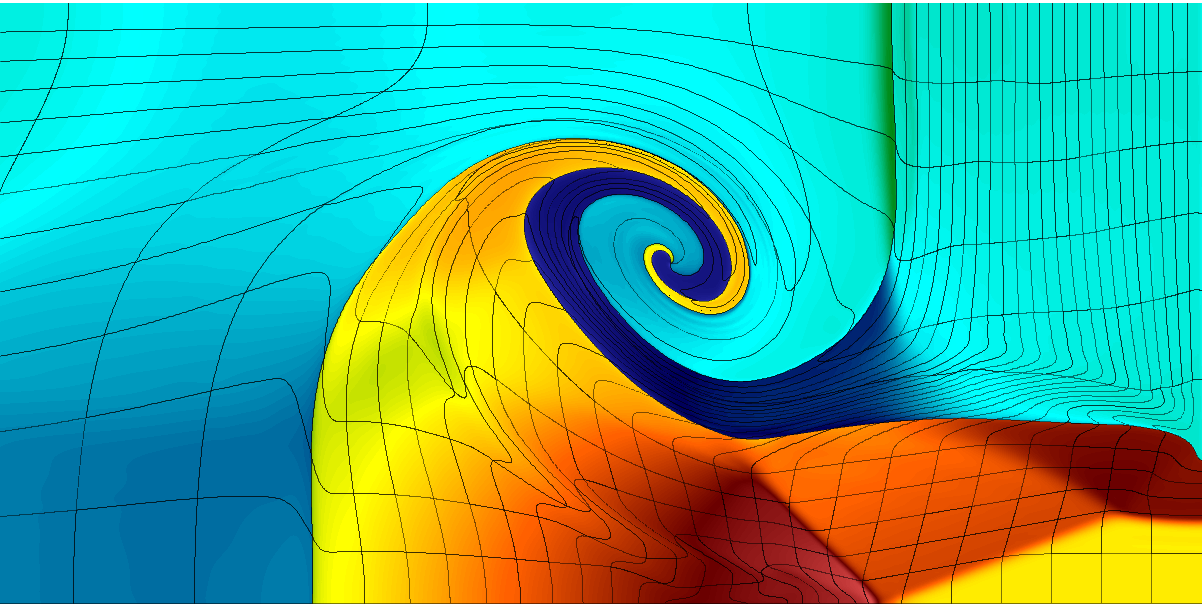
\includegraphics[scale = 0.15]{figs/triple-point_BLAST_q8q7.png} \\
            {\tiny Triple-Point problem with Q8-Q7}
          \end{tabular}
        \end{alertblock}
      \end{minipage}
    \end{center}
  \end{column}
  \begin{column}{0.30\textwidth}
    \begin{center}
      \begin{minipage}{0.95\textwidth}
        \begin{alertblock}{}
          \begin{center}
%          \begin{tabular}{c}
            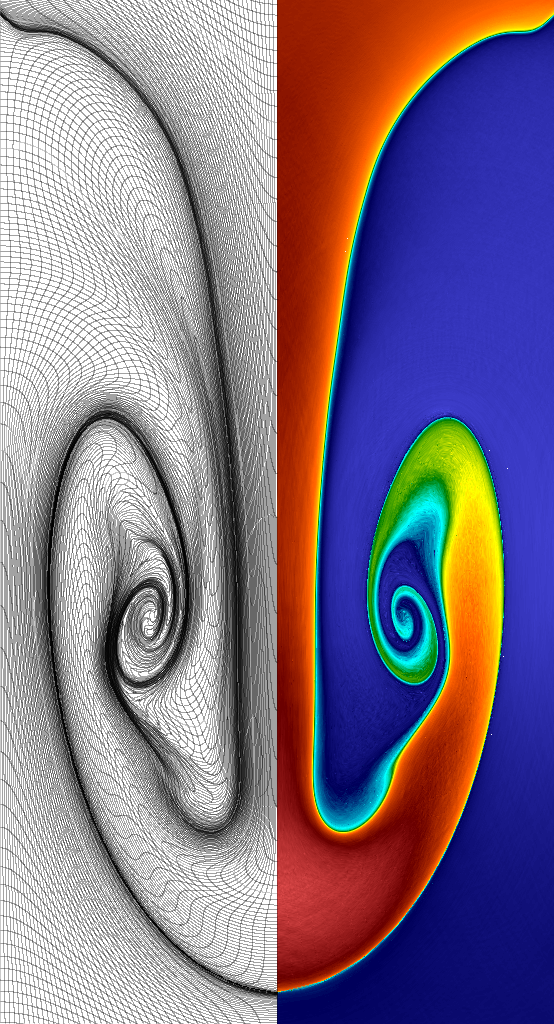
\includegraphics[scale = 0.1]{figs/q8q7_RT_density.png} \\
            {\tiny Rayleigh-Taylor Instability with Q8-Q7}
%          \end{tabular}
            \end{center}
      \end{alertblock}
    \end{minipage}
  \end{center}
\end{column}
\end{columns}

\begin{itemize}
\item \tiny{ https://computation.llnl.gov/casc/blast/blast.html}
\item \tiny{ Dobrev VA, Kolev TzV, Rieben RN. High order curvilinear finite element methods for Lagrangian hydrodynamics. SIAM J Sci Comput.}
\end{itemize}
\end{frame}
\begin{comment}
So what is BLAST? BLAST is a high order finite element hydrocode. We support
curvilinear elements which are able to bend and move with the fluid in a more
natural way than stock linear elements.

Kinematic variables (position, and velocity) are represented with continuous
fields, while thermodynamic variables (density, energy, pressure) use
discontinuous fields.

We achieve exact mass conservation by defining our density as a function of the
current jacobian of each element relative to it's original jacobian and
density.

This is all built on the open source mfem library and written in C++.

The algorithm is very FLOP intensive locally, allowing for very efficient
parallel implementations.
\end{comment}


%===============================================================================
% NEW SLIDE
%===============================================================================
\begin{frame}\frametitle{Artificial Viscosity in BLAST}
\begin{block}{}
{\small``Our idea is to introduce (artificial) dissipative terms into the
equations so as to give the shocks a thickness comparable to (but preferably
somewhat larger than) the spacing of the points of the network... Then the
differential equations ...may be used for the entire calculation, just as
though there were no shocks at all.'' -- Von Neumann and Richtmyer}\\
\end{block}
\bigskip

Ideally, an artifical viscosity implementation should:
\begin{itemize}
  \item Always reduces kinetic energy (dissipate shocks)
  \item Vanish in smooth regions and in rarefaction
  \item Vanish in uniform contraction and rigid rotation
  \item Satisfy Rankine-Hugoniot jump conditions away from the shock
  \item Be Galilean invariant

\bigskip
\begin{block}{Artificial Stress in BLAST}
\[
\sigma_a = \mu\frac{1}{2}(\nabla v+v\nabla)\,,\quad\text{where}\quad
\mu\equiv\rho(q_2l_s^2|\Delta_sv|+q_1l_sc_s)\,.
\]
\end{block}
\item This allows us to robustly handle shocks, but limits our convergence to first order in smooth flow.
\end{itemize}
\end{frame}
\begin{comment}
The longstanding problem with simulating the Euler equations is that shocks are
tricky.  They are infinitesimally thin, giving us no hopes of resolving them.
And these discontinuities can wreak havoc with high order methods, causing all
kinds of oscillations, typically referred to as Gibb's phenomenon. And since
the days of Von Neumann and Richtmyer, the accepted practice has been to
artificially add viscosity at shocks to smear them our and make them more
tenable to numerical simulation.

Unfortunately, there is not one correct way to implement artificial viscosity.
But an ideal implementation will have the following properties.

Obviously, it will dissipate our shocks.

It will go away when we don't want it there.

It will satisfy the Rankine-Hugoniot conditions.

And it must be Galilean invariant. We don't want to take one flow, add a
constant velocity to it, and get a different artificial viscosity.

Our current implementation of artificial viscosity in BLAST looks like this.
Our artificial stress is the product of an artificial viscosity and the
symmetric gradient of the velocity. And our artificial viscosity is some
function of the density, velocity, and sound speed.

In practice, this artificial viscosity has been pretty effective at robustly
simulating shock problems, but the artificial viscosity does not vanish in
smooth flow, which limits our convergence to first order.
\end{comment}


%===============================================================================
% NEW SLIDE
%===============================================================================
\begin{frame}\frametitle{Sub-Cell Shock Capturing of Persson and Peraire}
% Mention idea comes from Persson
\begin{itemize}
\item Shocks create oscillations in the highest polynomial modes.
\item Persson and Peraire
\footnote{P. Persson, J. Peraire, Sub-Cell Shock Capturing for Discontinuous
Galerkin Methods, 44th AIAA Aerospace Sciences Meeting and Exhibit, Reno,
Nevada, 2007. AIAA-2007-513}
do a change of basis to a hierarchical family of orthogonal polynomials, such that
\[
u=\sum_{i=1}^{N(k)}u_{i}\psi_i\,,
\]
where $u$ is some function of the solution (velocity, entropy, etc).
\item Define a truncated expansion
\[
\tilde u=\sum_{i=1}^{N(k-1)}u_{i}\psi_i\,.
\]
\item Compute a piece-wise constant smoothness indicator using numerical quadrature,
\[
s_z=\log_{10}\frac{(u-\tilde u,u-\tilde u)_z}{(u,u)_z}\,.
\]
\item Turn this into an artificial viscosity that vanishes for smooth, resolved flow.
\item In practice, this allows their high-order DG methods to achieve sub-zonal shock capturing.
\end{itemize}
\end{frame}
\begin{comment}
This work was very heavily inspired by some results that Per-Olof Persson
presented at the US National Congress on Computational Mechanics this July in
Raleigh. The basic ideas a kind of brilliant in their simplicity. We know that
shocks tend to excite the highest order modes of the solution. So why not use
that excitation as an indicator about where to put artificial viscosity.
Per-Olof uses high order discontinuous Galerkin methods to solve fluid
problems, so he is able to element-by-element do a change of basis to a
hierarchical orthogonal basis. He then uses the difference between the solution
and it's truncated expansion as a sort of shock detector, which he then
rescales to be an artificial viscosity. Note that I haven't defined what u is
yet, it could be any function of the solution, but some functions give better
results than others.
\end{comment}


%===============================================================================
% NEW SLIDE
%===============================================================================
\begin{frame}\frametitle{Multi-Resolution Viscosity Limiter in BLAST}
\begin{itemize}
\item Persson and Peraire use discontinuous spaces, which makes the orthogonal basis expansion straight-forward.
\item In BLAST, it makes more sense to do an $L^2$ projection using our continuous velocity space.
\item For $\mathbf{v}\in Q_k$, find $\mathbf{\tilde v}\in Q_{k-1}$ such that
\begin{align*}
\int_\Omega \mathbf{\tilde vw}dx&=\int_\Omega \mathbf{vw}dx\quad\forall \mathbf{w}\in Q_{k-1}\,.
\end{align*}
In matrix vector form, this is
\begin{align*}
\mathbf{M}_{k-1}\mathbf{\tilde v}&=\mathbf{g_v}\,.
\end{align*}
\item Use the difference as a shock detector which we call the smoothness.
\[
s_z=\log_{10}||\mathbf{v-\tilde v}||_z^2\,.
\]
\item Define a viscosity limiter,
\[
\psi_l=
\begin{cases}
0 &\text{if}\quad s_z <= s_0-\kappa\\
\frac{1}{2}\left(1+\sin\frac{\pi(s_z-s_0}{2\kappa}\right) &\text{if}\quad s_0-\kappa < s_z < s_0 + \kappa\\
1 &\text{if}\quad s_z >= s_0 + \kappa
\end{cases}
\]
where $s_0$ and $\kappa$ are tunable parameters that define the cutoff and transition region.
\item Use the new limited viscosity.
\[
\mu_l = \psi_l\mu
\]
\end{itemize}
\end{frame}
\begin{comment}
Based on our particular formulation in BLAST, we decided that the velocity
field might be the best option for shock detection. But since the velocity is
continuous, the orthogonal expansion is not quite so straight forward, so we
opted to do an L2 projection onto the lower order space instead.

So in finite element terminology, this looks like: Or in matrix vector format,
we get a familiar mass matrix times our unknown equals a RHS vector.

As per Per-Olof, we use the difference as a shock detector, but notice that we
have neglected the denominator term from his formulation. Since we are
triggering off of the velocity, the denominator would actually result in a
formulation that is not Galilean invariant. Apply a constant shift in the
velocity field would change the denominator, but leave the numerator unchanged.
The question of whether we should have some sort of denominator is still up for
discussion, however.

We now turn this smoothness value into a limiter. Any values below a certain
threshold are set to zero, while anything above another threshold are set to
one, with a transition region in between. It is now just left up to us to
choose appropriate s0 and kappa values.
\end{comment}


%===============================================================================
% NEW SLIDE
%===============================================================================
\begin{frame} \frametitle{High-order FEM overview: Time integration}
Let $Y = \left(\mathbf{v}; \mathbf{e}; \mathbf{x}\right)$. Then
the semi-discrete equations can be written in the form:
\vspace{-2.5mm}
\begin{columns}
\begin{column}{0.3\textwidth}
  \begin{center}
  \begin{minipage}{0.8\textwidth}
  \begin{block}{}
  \centering
  $\dfrac{\dd Y}{\dd t} = \mathcal{F}(Y, t)$
  \end{block}
  \end{minipage}
  \end{center}
\end{column}
\begin{column}{0.7\textwidth}
  \begin{center}
  \begin{minipage}{0.8\textwidth}
  \begin{alertblock}{}
  \centering
  $
    \mathcal{F}(Y, t) =
    \begin{pmatrix}
    \mathcal{F}_v(\mathbf{v}, \mathbf{e}, \mathbf{x}) \\
    \mathcal{F}_e(\mathbf{v}, \mathbf{e}, \mathbf{x}) \\
    \mathcal{F}_x(\mathbf{v}, \mathbf{e}, \mathbf{x})\\
    \end{pmatrix}
    =
    \begin{pmatrix}
    - \mathbf{M_v}^{\!\!-1} \mathbf{F}\cdot \mathbf{1} \\
    \mathbf{M_e}^{\!\!-1} \mathbf{F}^\top \cdot \mathbf{v} \\
    \mathbf{v}\\
    \end{pmatrix}
  $
  \end{alertblock}
  \end{minipage}
  \end{center}
\end{column}
\end{columns}
\medskip
Standard high-order time integration techniques (e.g.\ explicit Runge-Kutta
methods) can be applied to this system of nonlinear ODEs.

\medskip

The $L^2$ projection is done at each stage of the integration and used in the artificial viscosity when computing $\mathbf{F}$.

\medskip

For example, consider the \myem{energy conserving} RK2Avg method:
\begin{center}
\begin{minipage}[c]{0.425\textwidth}\begin{alertblock}{}\centering
$
\begin{aligned}
\mathbf{\tilde v} &= \mathbf{M}_{k-1}^{-1}\mathbf{g_v}\\
\mathbf{v}^{n+\frac{1}{2}} &= \mathbf{v}^{n} - (\Delta t/2)\, \mathbf{M_v}^{\!\!-1} \mathbf{F}^n\cdot \mathbf{1} \\
\mathbf{e}^{n+\frac{1}{2}} &= \mathbf{e}^{n} + (\Delta t/2)\, \mathbf{M_e}^{\!\!-1} (\mathbf{F}^n)^\top \cdot \mathbf{v}^{n+\frac{1}{2}} \\
\mathbf{x}^{n+\frac{1}{2}} &= \mathbf{x}^{n} + (\Delta t/2)\, \mathbf{v}^{n+\frac{1}{2}}\\
\end{aligned}
$
\end{alertblock}\end{minipage}
\hspace{0.09\textwidth}
\begin{minipage}[c]{0.425\textwidth}\begin{alertblock}{}\centering
$
\begin{aligned}
\mathbf{\tilde v} &= \mathbf{M}_{k-1}^{-1}\mathbf{g_v}\\
\mathbf{v}^{n+1} &= \mathbf{v}^{n} - \Delta t\,  \mathbf{M_v}^{\!\!-1} \mathbf{F}^{n+\frac{1}{2}}\cdot \mathbf{1} \\
\mathbf{e}^{n+1} &= \mathbf{e}^{n} + \Delta t\,  \mathbf{M_e}^{\!\!-1} (\mathbf{F}^{n+\frac{1}{2}})^\top \cdot \bar{\mathbf{v}}^{n+\frac{1}{2}} \\
\mathbf{x}^{n+1} &= \mathbf{x}^{n} +  \Delta t\, \bar{\mathbf{v}}^{n+\frac{1}{2}}\\
\end{aligned}
$
\end{alertblock}\end{minipage}
\end{center}
\end{frame}
\begin{comment}
Here, we can see our entire BLAST algorithm distilled into compact form. Basically,
we end up with a system of nonlinear ODEs in time that we can integrate with
high order techniques.

The key change we now have to deal with is that prior to computing the corner forces
at each stage, we need to do our low order projection, which will be used in the
computation of the artificial viscosity.
\end{comment}


%===============================================================================
% NEW SLIDE
%===============================================================================
\begin{frame}\frametitle{Taylor Green Vortex, $s_0=-11$, $\kappa=1$}
\begin{itemize}
\item On coarse meshes, the indicator does not detect sufficient smoothness
in the solution to turn off viscosity.
\item With sufficient resolution, the indicator shuts down all viscosity and we
recover higher order convergence rates.
\end{itemize}
\begin{columns}
\begin{column}{0.25\textwidth}
\centering{Q2-Q1}
\vspace{-4ex}
\begin{figure}[t]
\begin{center}
\includegraphics<1>[height=0.8\textwidth]{figs/TG-2/Q2-smoothness-4.png}
\includegraphics<2>[height=0.8\textwidth]{figs/TG-2/Q2-smoothness-5.png}
\includegraphics<3>[height=0.8\textwidth]{figs/TG-2/Q2-smoothness-6.png}
\includegraphics<4>[height=0.8\textwidth]{figs/TG-2/Q2-smoothness-7.png}
\small{\\Smoothness}
\end{center}
\end{figure}
\begin{figure}[t]
\begin{center}
\includegraphics<1>[height=0.8\textwidth]{figs/TG-2/Q2-limiter-4.png}
\includegraphics<2>[height=0.8\textwidth]{figs/TG-2/Q2-limiter-5.png}
\includegraphics<3>[height=0.8\textwidth]{figs/TG-2/Q2-limiter-6.png}
\includegraphics<4>[height=0.8\textwidth]{figs/TG-2/Q2-limiter-7.png}
\small{\\Limiter}
\end{center}
\end{figure}
\end{column}
\begin{column}{0.25\textwidth}
\centering{Q4-Q3}
\vspace{-4ex}
\begin{figure}[t]
\begin{center}
\includegraphics<1>[height=0.8\textwidth]{figs/TG-2/Q4-smoothness-4.png}
\includegraphics<2>[height=0.8\textwidth]{figs/TG-2/Q4-smoothness-5.png}
\includegraphics<3>[height=0.8\textwidth]{figs/TG-2/Q4-smoothness-6.png}
\includegraphics<4>[height=0.8\textwidth]{figs/TG-2/Q4-smoothness-7.png}
\small{\\Smoothness}
\end{center}
\end{figure}
\begin{figure}[t]
\begin{center}
\includegraphics<1>[height=0.8\textwidth]{figs/TG-2/Q4-limiter-4.png}
\includegraphics<2>[height=0.8\textwidth]{figs/TG-2/Q4-limiter-5.png}
\includegraphics<3>[height=0.8\textwidth]{figs/TG-2/Q4-limiter-6.png}
\includegraphics<4>[height=0.8\textwidth]{figs/TG-2/Q4-limiter-7.png}
\small{\\Limiter}
\end{center}
\end{figure}
\end{column}
\begin{column}{0.5\textwidth}
\begin{figure}[t]
\begin{center}
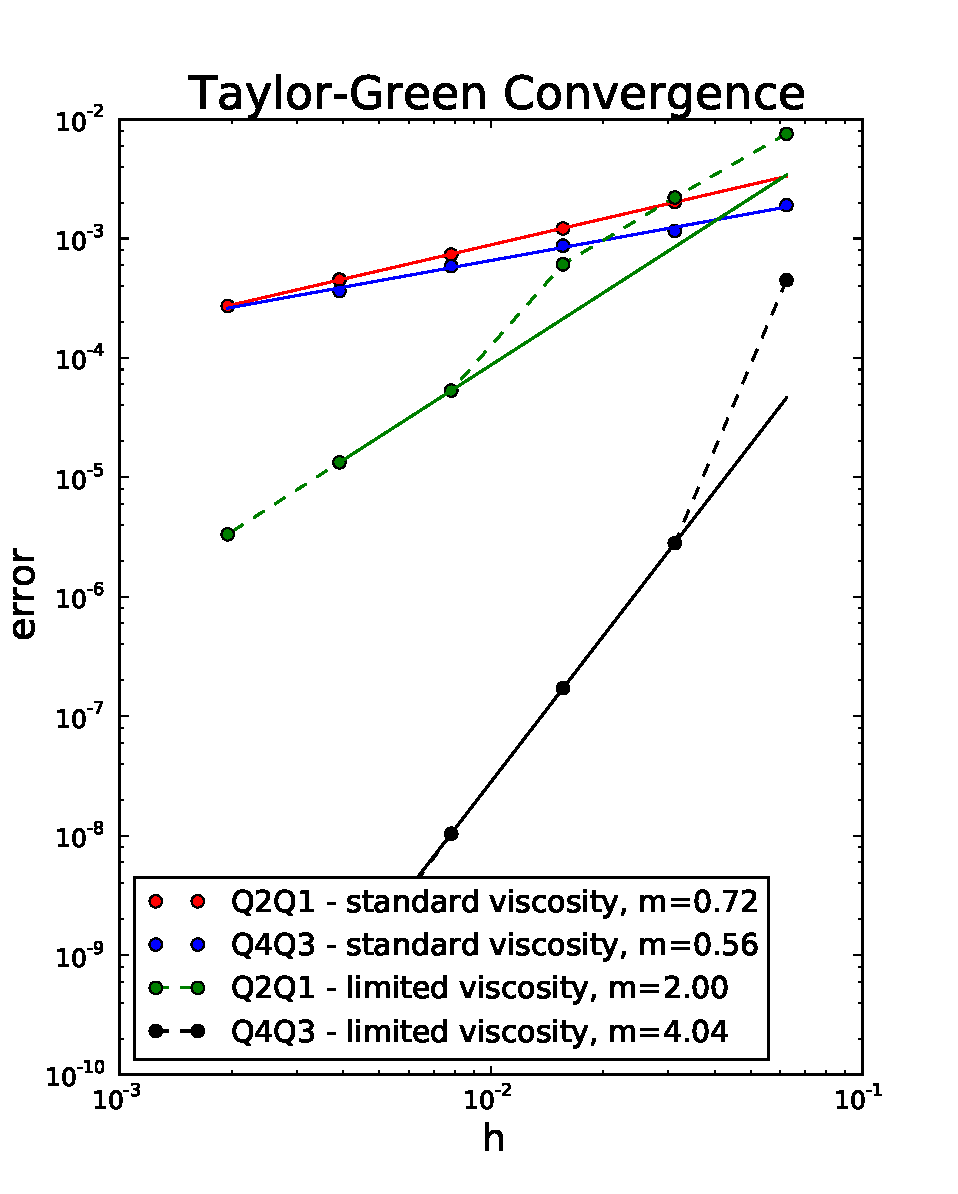
\includegraphics[width=0.8\textwidth]{figs/TGConvergence.pdf}
\end{center}
\end{figure}
\end{column}
\end{columns}
\end{frame}
\begin{comment}
So let's see how our new viscosity limiter works on a few test problems.  The
first promise I made was that our viscosity limiter should allow us to recover
higher order convergence on smooth problems. Here we have the Taylor-Green
vortex, which is a smooth steady state solution for the Euler equations. So the
initial condition is the exact solution. We just propogate forward to a certain
time and measure the amount of error that has polluted our solution.

As you can see on the convergence chart, the standard viscosity is giving less
than first order convergence, even with second and fourth order methods. You
can see the smoothness plots for Q2-Q1 and Q4-Q3 elements on the same initial
mesh. You can see that our indicator is starting to turn off viscosity in the
smoother parts of the flow for Q4, but it does not yet detect sufficient
smoothness in the Q2 results to do so.

With one more refinement, the indicator has turned off all viscosity in the Q4
results, and it is just starting to notice it can turn off some of the Q2
viscosity.

With another refinement, it is turning off large swaths of viscosity in Q2,
while Q4 will continue to remain off.

With another refinement, we see that Q2 viscosity is almost completely off, and
a further refinement will achieve full elimination of viscosity.

Let me quickly point out that these values of s0 and kappa are very
conservative.  They were chosen earlier on as the strictest values to allow us
to deal with every problem we had considered at that point. We recently
discovered that we could get away with looser values on most problems, as the
following slides will demonstrate.  But these Taylor Green results were the
most time consuming to generate, so I haven't had time to rerun our results
with the new values.

As you can see on the convergence chart, after a couple data points where
sufficient resolution is not detected, we are able to achieve our higher order
convergence.
\end{comment}


%===============================================================================
% NEW SLIDE
%===============================================================================
\begin{frame}\frametitle{Sod Shock Tube, $s_0=-9.5$, $\kappa=0.5$}
\vspace{-1ex}
Q4-Q3 elements on a 50x1 mesh
\vspace{-2ex}
\begin{columns}
\begin{column}{0.3\textwidth}
\begin{figure}[t]
\begin{center}
Smoothness
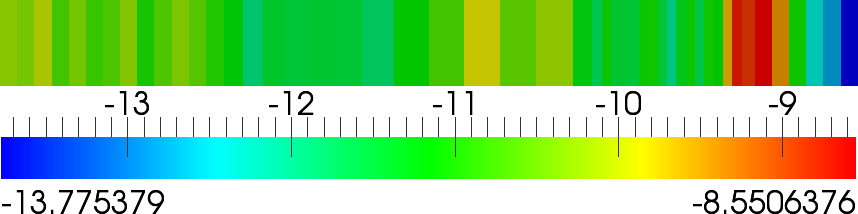
\includegraphics[width=1.0\textwidth]{figs/Sod/Q4l-50-smoothness.png}
\end{center}
\end{figure}
\begin{figure}[t]
\begin{center}
Limiter
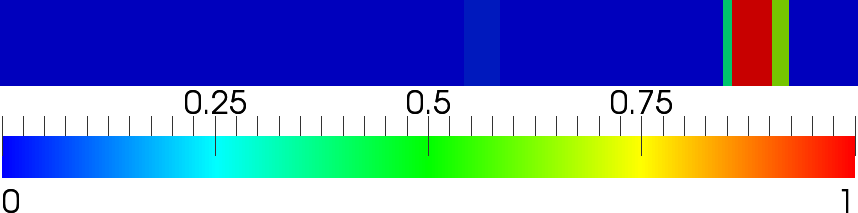
\includegraphics[width=1.0\textwidth]{figs/Sod/Q4l-50-limiter.png}
\end{center}
\end{figure}
\begin{figure}[t]
\begin{center}
Viscosity with Limiter
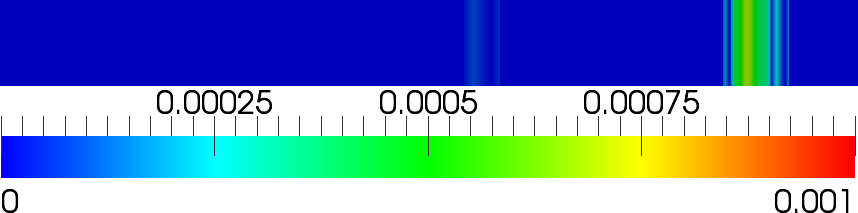
\includegraphics[width=1.0\textwidth]{figs/Sod/Q4l-50-viscosity.png}
\end{center}
\end{figure}
\begin{figure}[t]
\begin{center}
Viscosity without Limiter
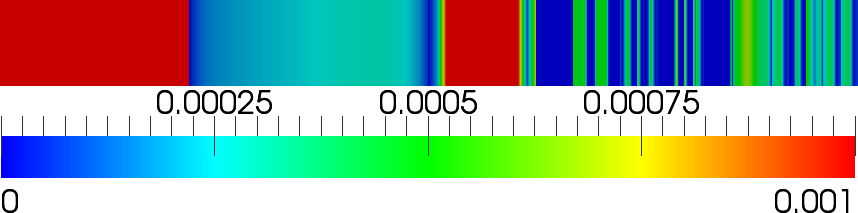
\includegraphics[width=1.0\textwidth]{figs/Sod/Q4nl-50-viscosity.png}
\end{center}
\end{figure}
\end{column}
\begin{column}{0.7\textwidth}
\begin{center}
% Density\\
\includegraphics<1>[width=0.8\textwidth]{figs/Sod/Q4-50-Density.png}
\includegraphics<2>[width=0.8\textwidth]{figs/Sod/Q4-50-Density-zoom.png}
\end{center}
\end{column}
\end{columns}
\end{frame}
\begin{comment}
Now that we know we are able to get rid of viscosity when we don't need it, we
need to make sure we can keep it when we do. So here we have the Sod shock
tube.  Looking at the exact solution from the right to the left, we have a low
density fluid, then a shock traveling to the right, a material interface with a
higher density fluid, and then a rarefaction wave moving to the left. We really
only want our viscosity to trigger on the shock since the material interface
isn't an actual shock.

You can see the computed smoothness field on the top left. And as I promised
earlier, it is a fairly reliable indicator of where the shock is. It doesn't
even pick up on the material interface. Also, our limiter below is very
exclusive about where it turns on viscosity. On the bottom, you can see what
our viscosity field looks like without a limiter. We get a lot of viscosity in
non-shocked regions, which is not what we want.

But if you look at the plot on the right, you can see that it doesn't appear to
be hurting us too much. If we zoom in, you can see that the viscosity limited
solution is a little closer in the rarefaction wave, but not significantly. The
main takeaway of course, is that our standard implementation seems to do
alright even if it does produce unnecessary viscosity.
\end{comment}


%===============================================================================
% NEW SLIDE
%===============================================================================
\begin{frame}\frametitle{Sedov Blast Wave, $s_0=-9.5$, $\kappa=0.5$}
\vspace{1ex}
Q2-Q1 elements on an 80x80 mesh
\vspace{-4ex}
\begin{columns}
\begin{column}{0.3\textwidth}
\begin{figure}[t]
\begin{center}
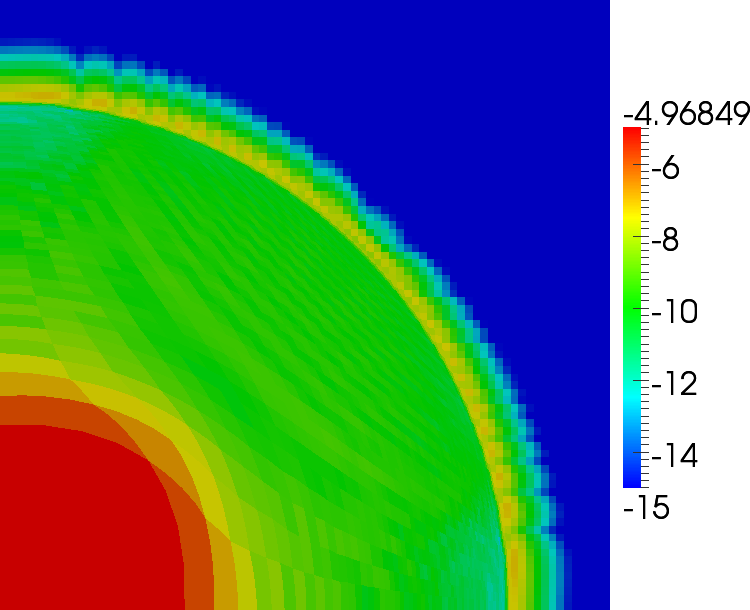
\includegraphics[height=0.9\textwidth]{figs/Sedov/Q2l-80-smoothness.png}
\\Smoothness
\end{center}
\end{figure}
\begin{figure}[t]
\begin{center}
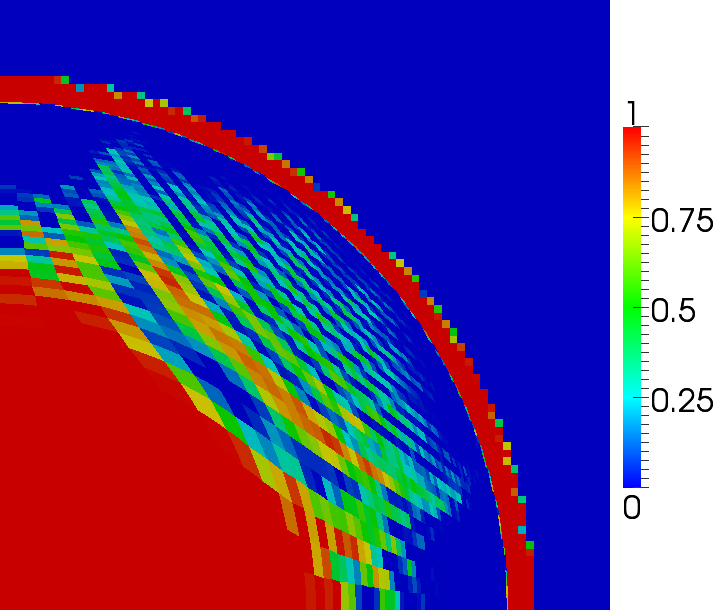
\includegraphics[height=0.9\textwidth]{figs/Sedov/Q2l-80-limiter.png}
\\Limiter
\end{center}
\end{figure}
\end{column}
\begin{column}{0.3\textwidth}
\begin{figure}[t]
\begin{center}
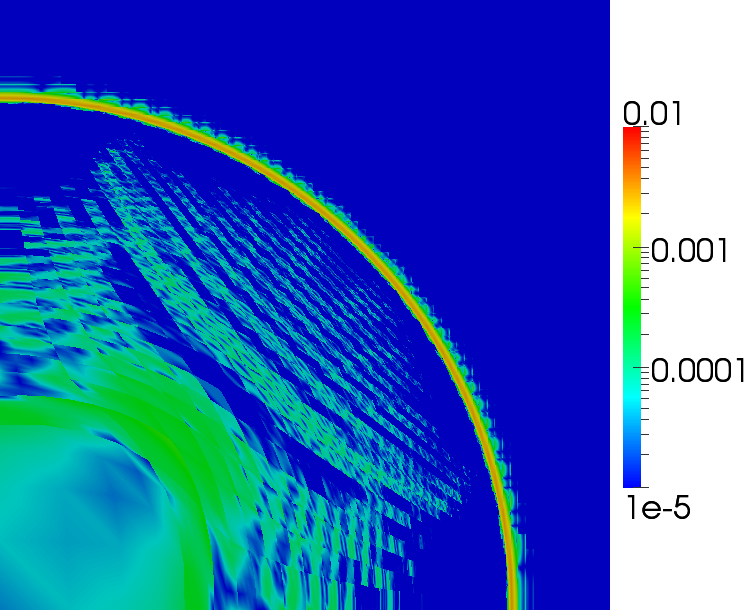
\includegraphics[height=0.9\textwidth]{figs/Sedov/Q2l-80-viscosity.png}
\\Viscosity with Limiter
\end{center}
\end{figure}
\begin{figure}[t]
\begin{center}
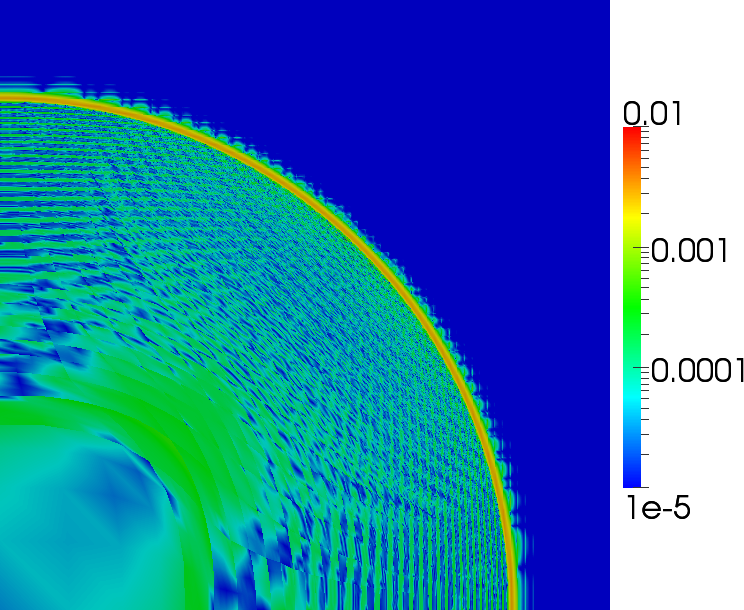
\includegraphics[height=0.9\textwidth]{figs/Sedov/Q2nl-80-viscosity.png}
\\Viscosity without Limiter
\end{center}
\end{figure}
\end{column}
\begin{column}{0.3\textwidth}
\begin{figure}[t]
\begin{center}
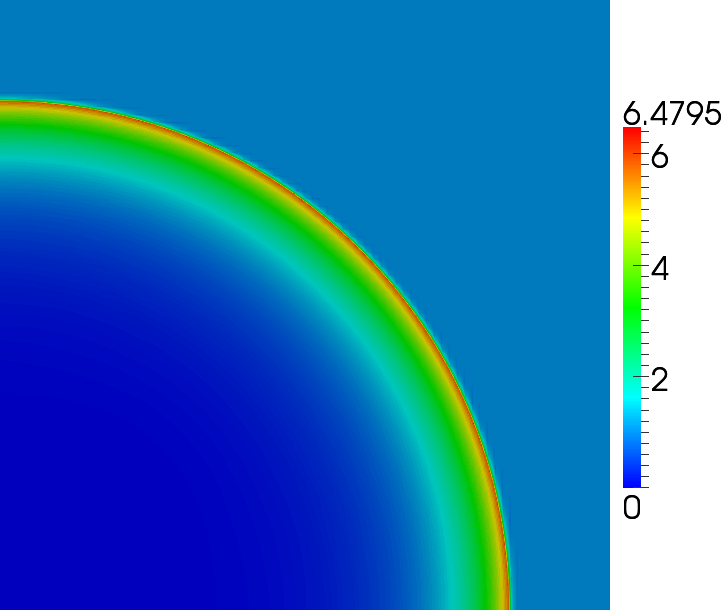
\includegraphics[height=0.9\textwidth]{figs/Sedov/Q2l-80-density.png}
\\Density with Limiter
\end{center}
\end{figure}
\begin{figure}[t]
\begin{center}
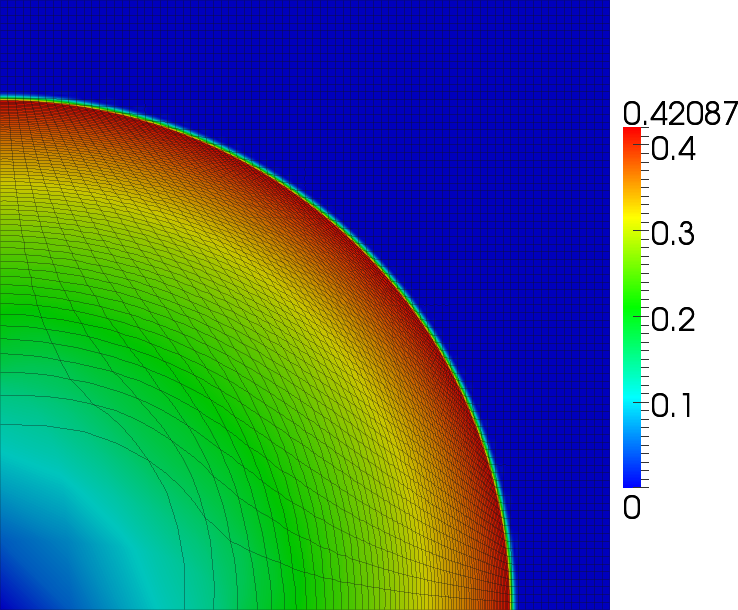
\includegraphics[height=0.9\textwidth]{figs/Sedov/Q2l-80-velocity.png}
\\Velocity with Limiter
\end{center}
\end{figure}
\end{column}
\end{columns}
\end{frame}
\begin{comment}
Here we have the Sedov blast wave. Basically an explosion that propogates
outward.  You can see that the smoothness seems to trigger pretty strongly at
the origin and at the shock. The shock is expected, but you kind of have to
think for a while before you realize why the origin is being triggered. That
first zone has expanded so much, that the basis functions have to handle a good
amount of physics within one cell. The projection from Q2 to Q1 is not close to
sufficient, and the difference is substantial.  So we do end up maintaining a
good amount of viscosity at the origin. We might expect our limiter to be more
discerning with a higher order method, but we still need to run a few more
experiments.

In any case, we do manage to kill some of the post shock viscosity while
maintaining a pretty solid solution.
\end{comment}


%===============================================================================
% NEW SLIDE
%===============================================================================
\begin{frame}\frametitle{Noh Implosion, $s_0=-9.5$, $\kappa=0.5$}
\vspace{1ex}
Q2-Q1 elements on an 128x128 mesh
\vspace{-4ex}
\begin{columns}
\begin{column}{0.3\textwidth}
\begin{figure}[t]
\begin{center}
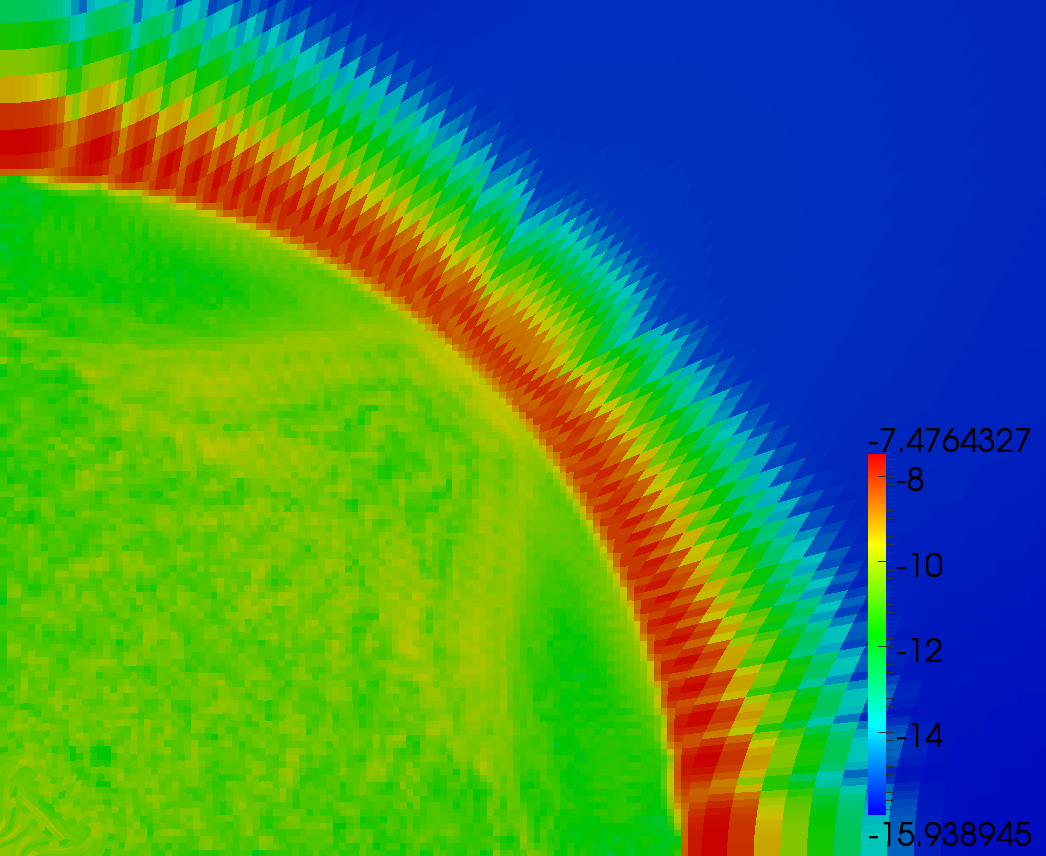
\includegraphics[height=0.9\textwidth]{figs/Noh/Q2l-7-smoothness.png}
\\Smoothness
\end{center}
\end{figure}
\begin{figure}[t]
\begin{center}
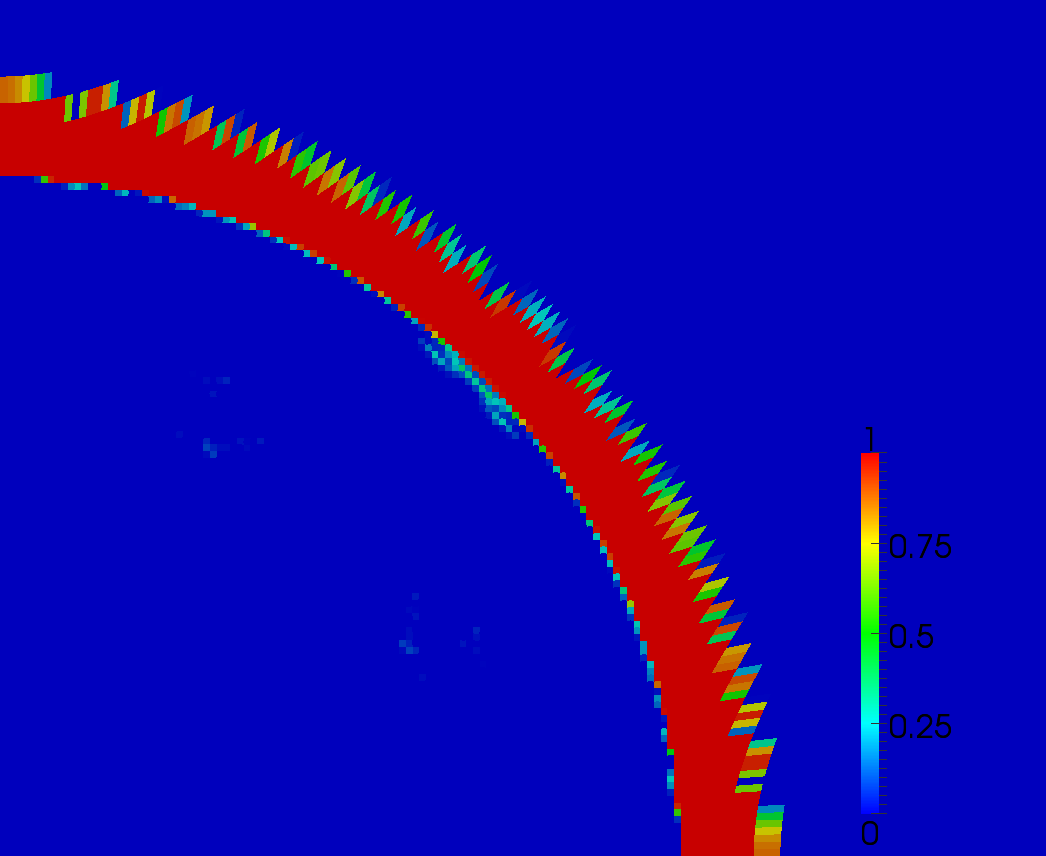
\includegraphics[height=0.9\textwidth]{figs/Noh/Q2l-7-limiter.png}
\\Limiter
\end{center}
\end{figure}
\end{column}
\begin{column}{0.3\textwidth}
\begin{figure}[t]
\begin{center}
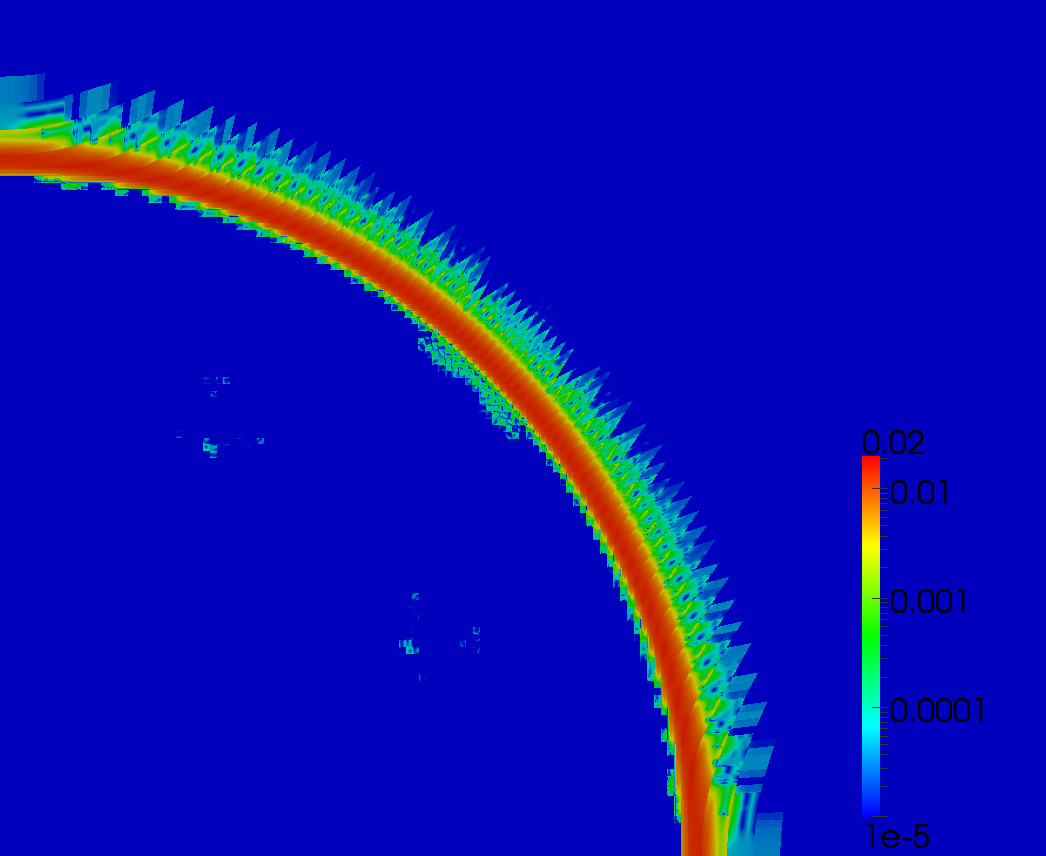
\includegraphics[height=0.9\textwidth]{figs/Noh/Q2l-7-viscosity.png}
\\Viscosity with Limiter
\end{center}
\end{figure}
\begin{figure}[t]
\begin{center}
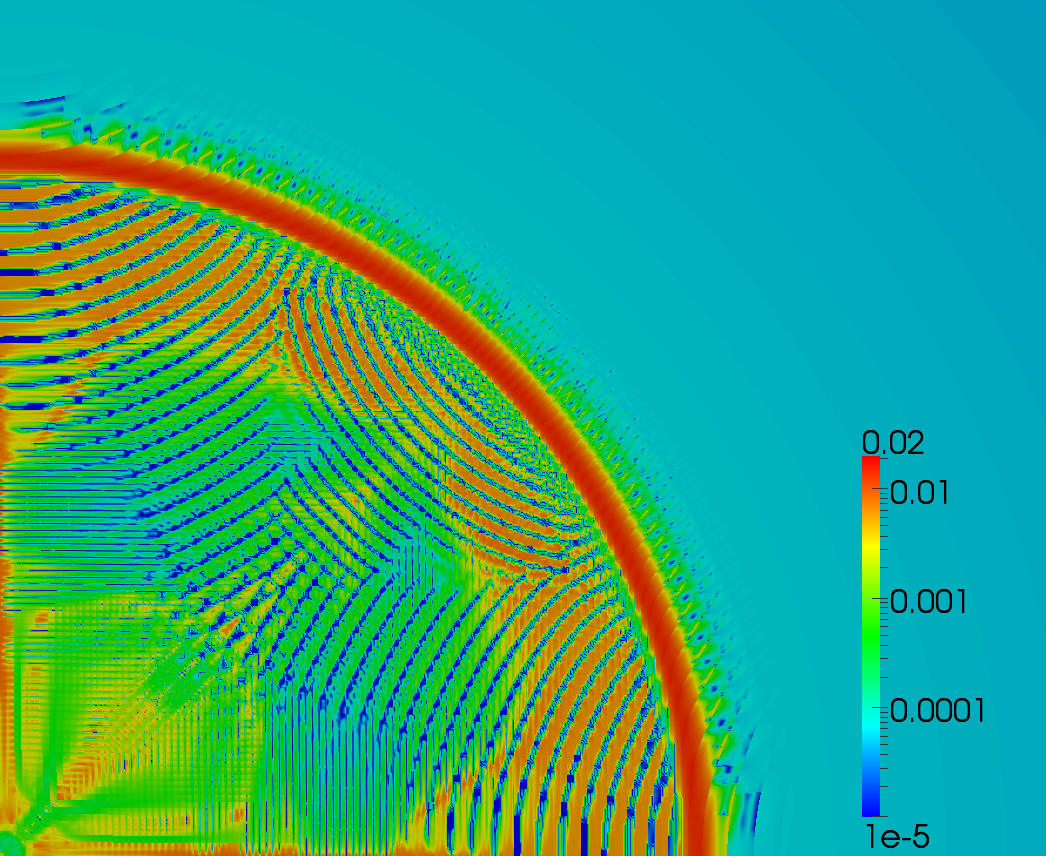
\includegraphics[height=0.9\textwidth]{figs/Noh/Q2nl-7-viscosity.png}
\\Viscosity without Limiter
\end{center}
\end{figure}
\end{column}
\begin{column}{0.3\textwidth}
\begin{figure}[t]
\begin{center}
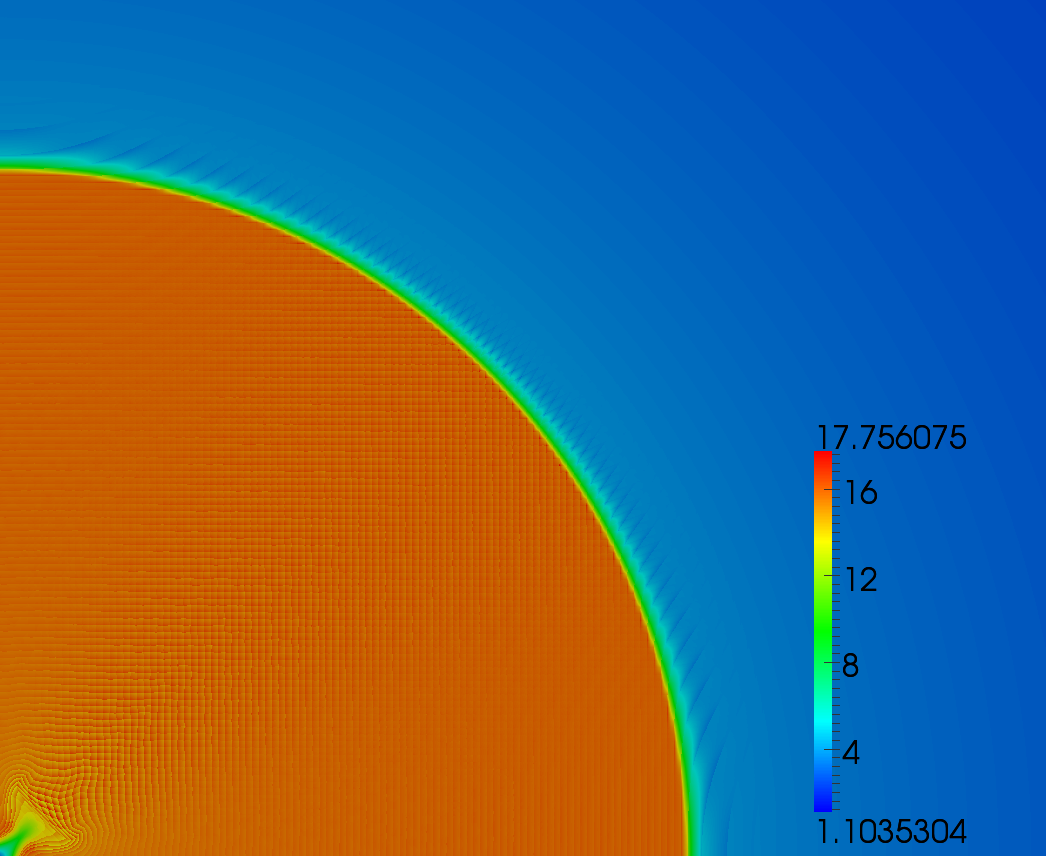
\includegraphics[height=0.9\textwidth]{figs/Noh/Q2l-7-density.png}
\\Density with Limiter
\end{center}
\end{figure}
\begin{figure}[t]
\begin{center}
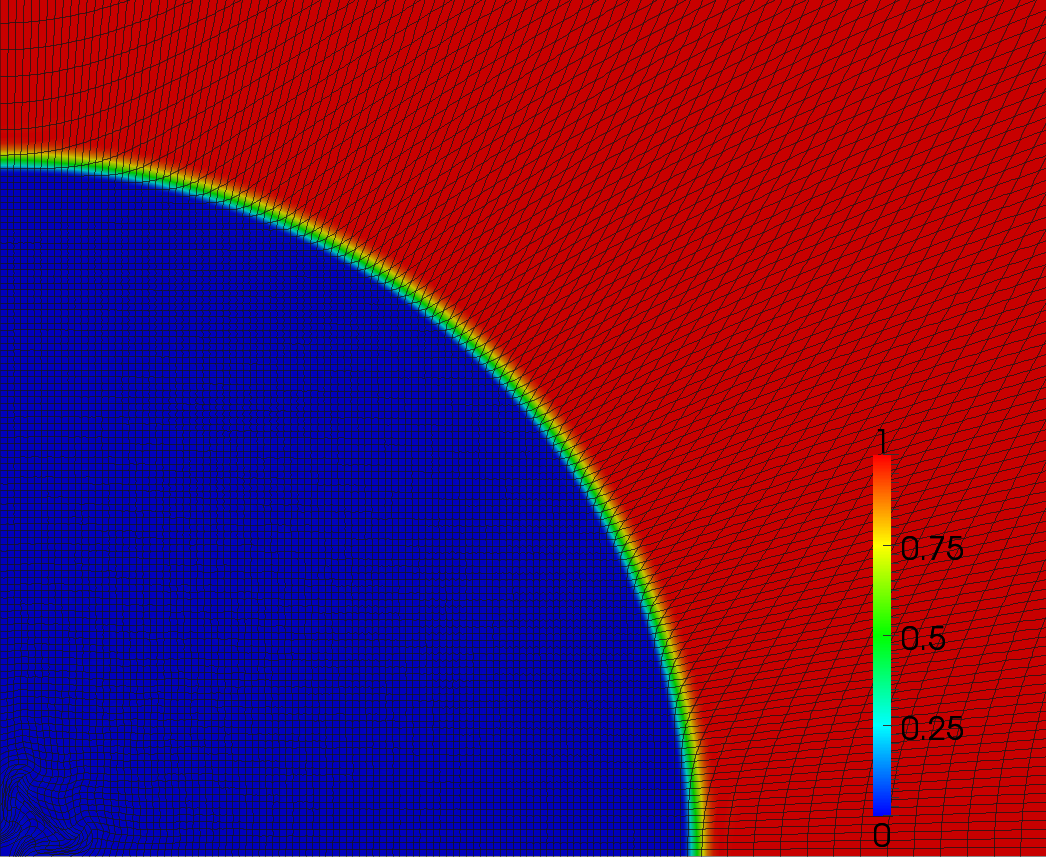
\includegraphics[height=0.9\textwidth]{figs/Noh/Q2l-7-velocity.png}
\\Velocity with Limiter
\end{center}
\end{figure}
\end{column}
\end{columns}
\end{frame}
\begin{comment}
The Noh implosion is just a very hard problem. We have to deal with this weird
phenomenon known as wall heating which occurs at the origin and really degrades
the accuracy of simulations. And unfortunately for us, extra viscosity post
shock can make things a little nicer. That's the problem with getting rid of
viscosity. Viscosity is nice, and always makes things smoother and nicer
looking. But smooth, nice looking solutions don't always reflect reality. So we
have to be careful when judging solutions qualitatively based on how nice they
look. Sometimes real flows don't look nice. I'm not saying that this weird
tangled stuff at the origin is good, but we have larger issues going on with
Noh that degrade the solution. Normally we would want to get rid of post-shock
viscosity.
\end{comment}


%===============================================================================
% NEW SLIDE
%===============================================================================
\begin{frame}\frametitle{Noh Implosion, $s_0=-9.5$, $\kappa=0.5$}
\begin{columns}
\begin{column}{0.35\textwidth}
\begin{center}
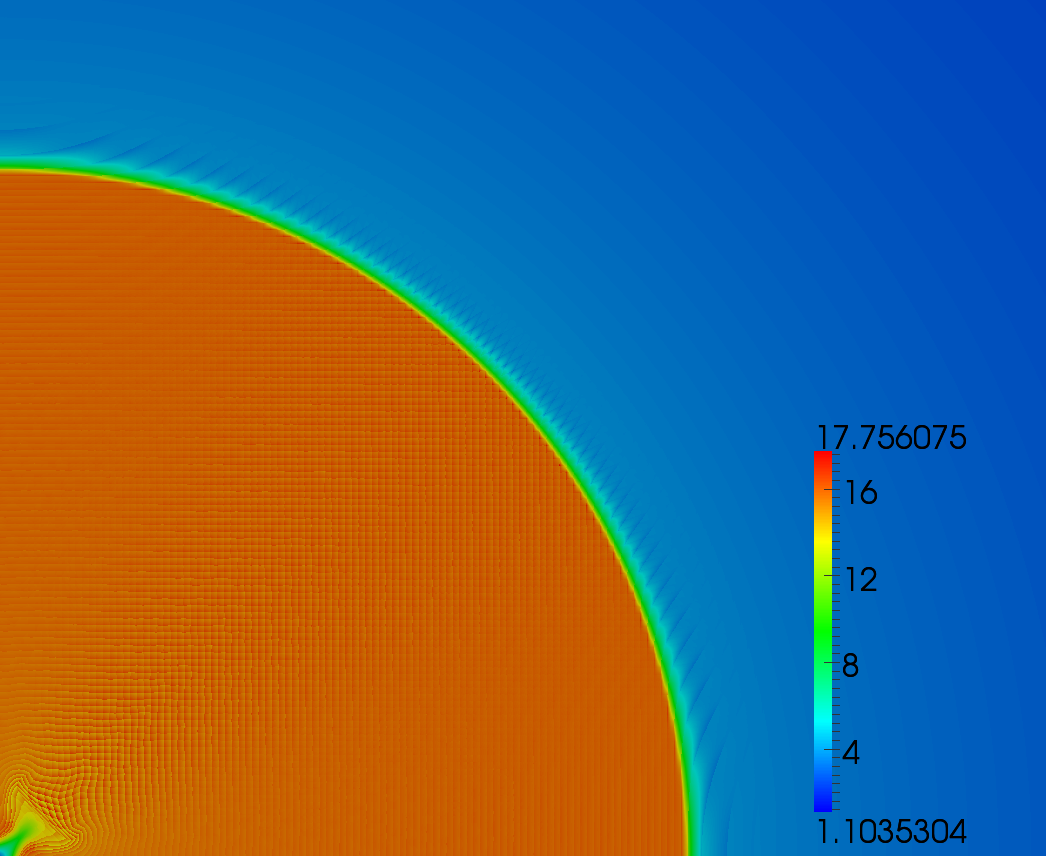
\includegraphics[height=0.9\textwidth]{figs/Noh/Q2l-7-density.png}
\\Density with Limiter
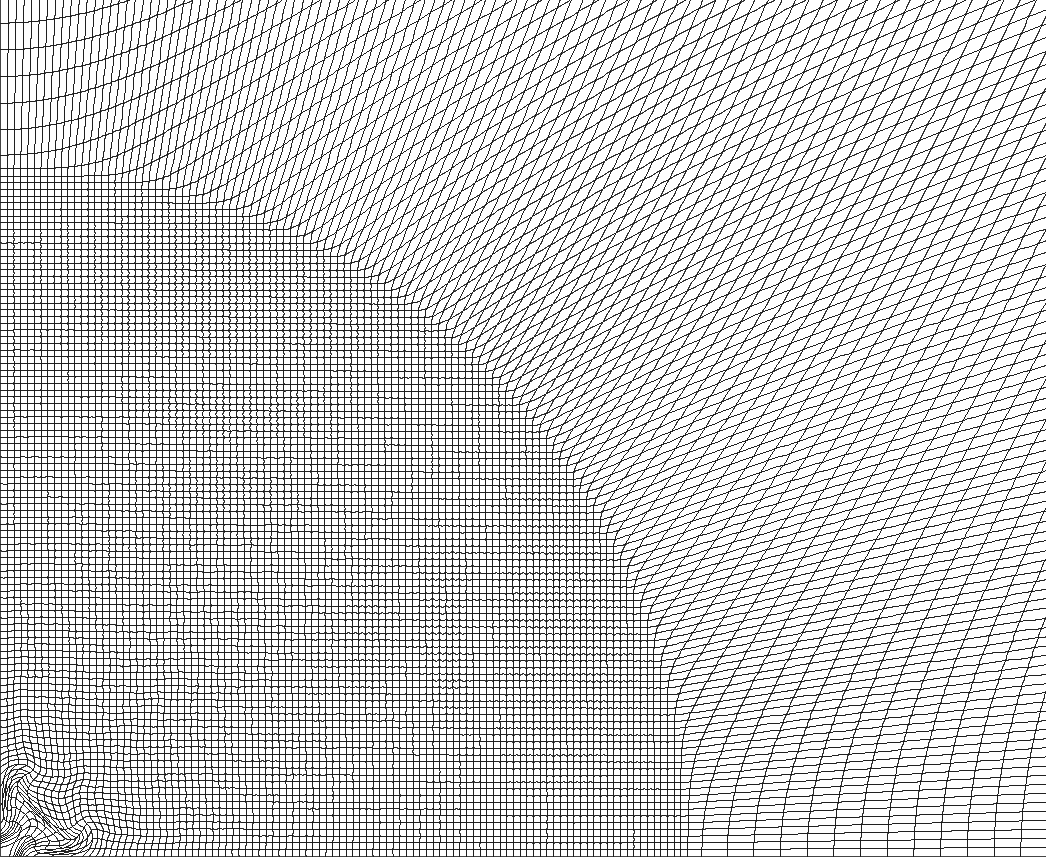
\includegraphics[height=0.9\textwidth]{figs/Noh/Q2l-7-mesh.png}
\\Mesh with Limiter
\end{center}
\end{column}
\begin{column}{0.35\textwidth}
\begin{center}
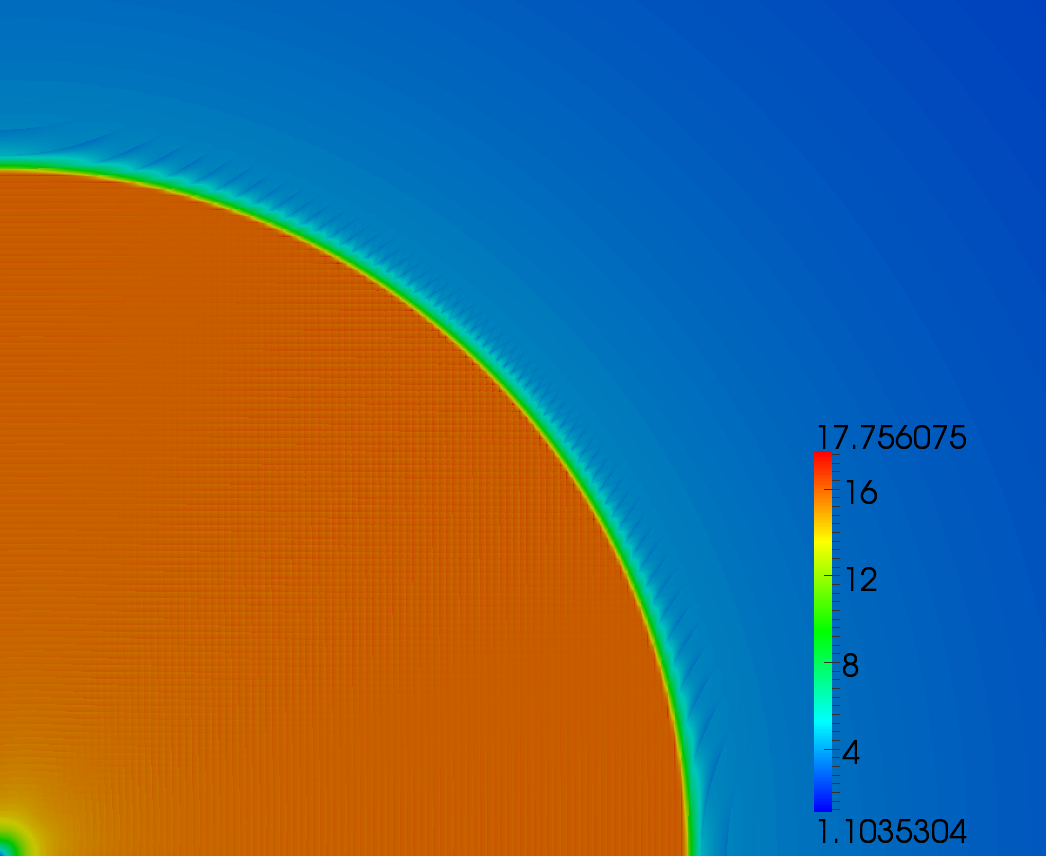
\includegraphics[height=0.9\textwidth]{figs/Noh/Q2nl-7-density.png}
\\Density without Limiter
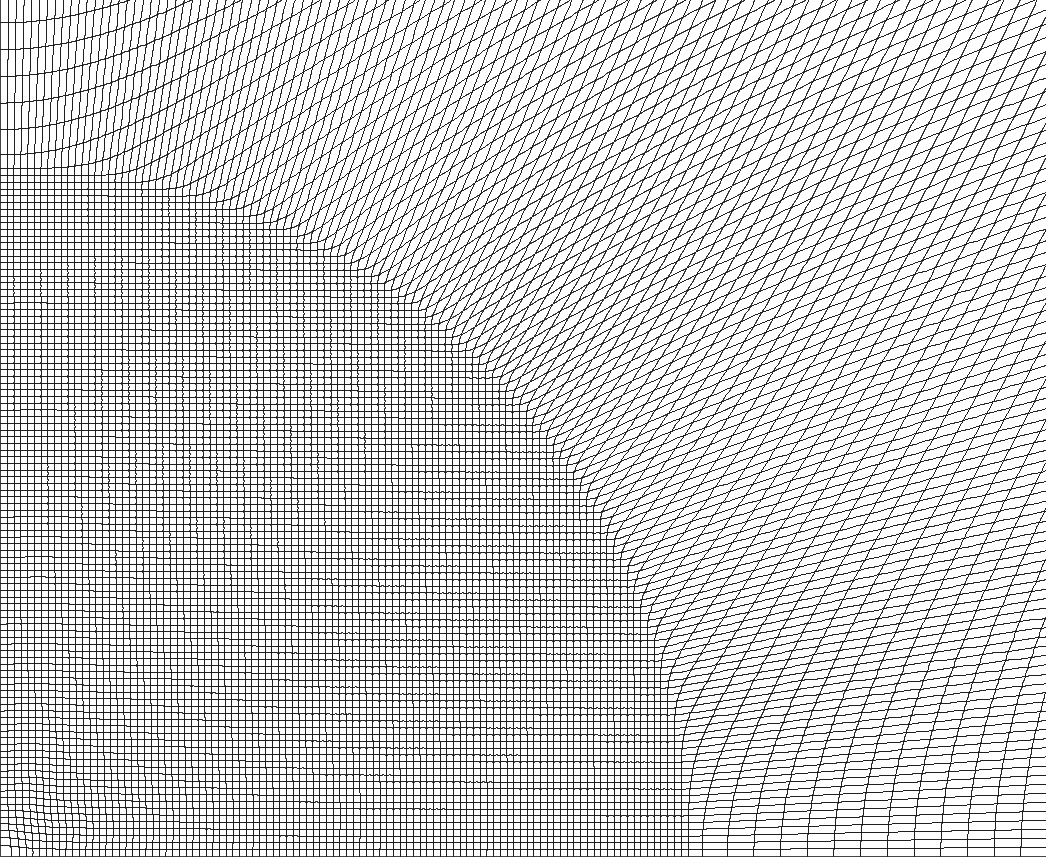
\includegraphics[height=0.9\textwidth]{figs/Noh/Q2nl-7-mesh.png}
\\Mesh without Limiter
\end{center}
\end{column}
\end{columns}
\end{frame}


%===============================================================================
% NEW SLIDE
%===============================================================================
\begin{frame}\frametitle{Triple Point Shockwave, $s_0=-9.5$, $\kappa=0.5$}
\vspace{1ex}
% Q2-Q1 elements
\vspace{-4ex}
\small{
\begin{columns}
\begin{column}{0.45\textwidth}
\begin{center}
Smoothness\\
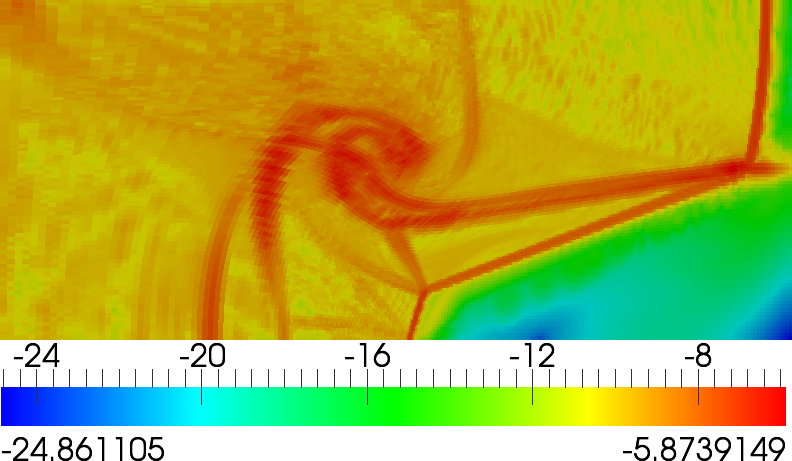
\includegraphics[width=0.8\textwidth]{figs/TriplePt/Q2-4-smoothness-limiter.png}\\
Viscosity with Limiter\\
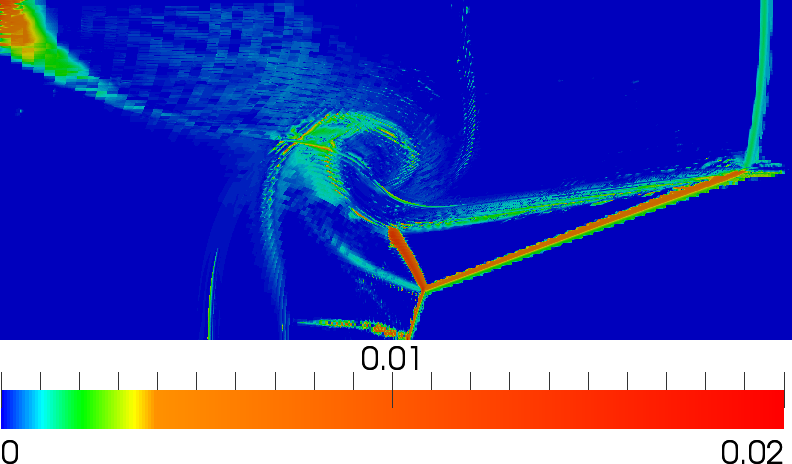
\includegraphics[width=0.8\textwidth]{figs/TriplePt/Q2-4-viscosity-limiter.png}\\
Density with Limiter\\
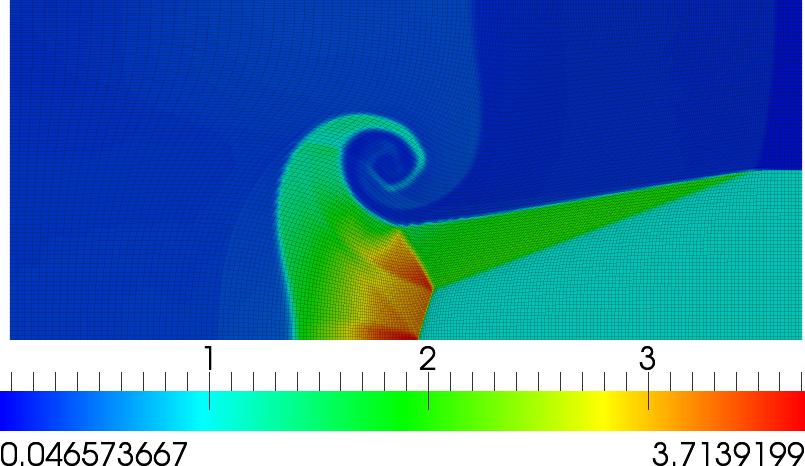
\includegraphics[width=0.8\textwidth]{figs/TriplePt/Q2-4-density-limiter.png}\\
\end{center}
\end{column}
\begin{column}{0.45\textwidth}
\begin{center}
Limiter\\
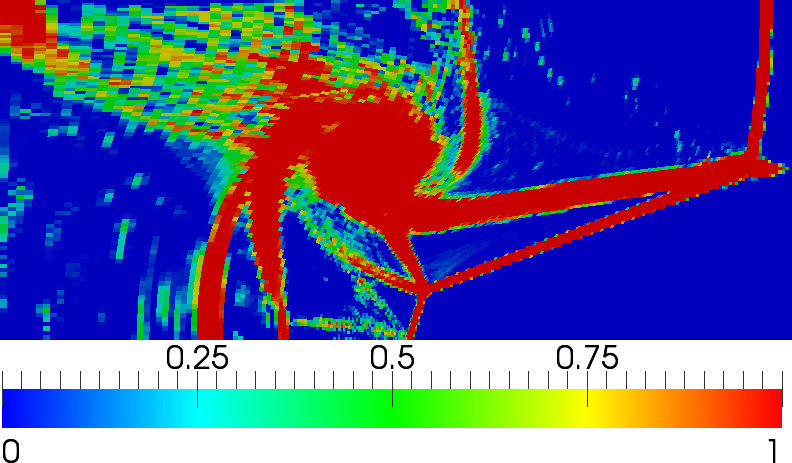
\includegraphics[width=0.8\textwidth]{figs/TriplePt/Q2-4-limiter-limiter.png}\\
Viscosity without Limiter\\
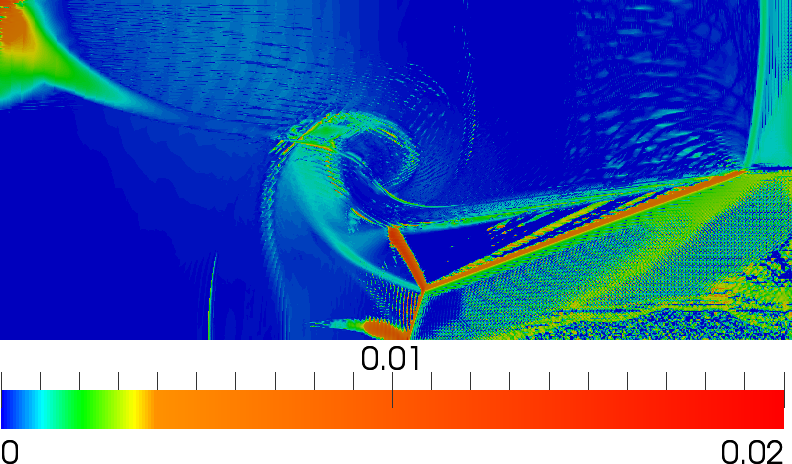
\includegraphics[width=0.8\textwidth]{figs/TriplePt/Q2-4-viscosity-nolimiter.png}\\
Density without Limiter\\
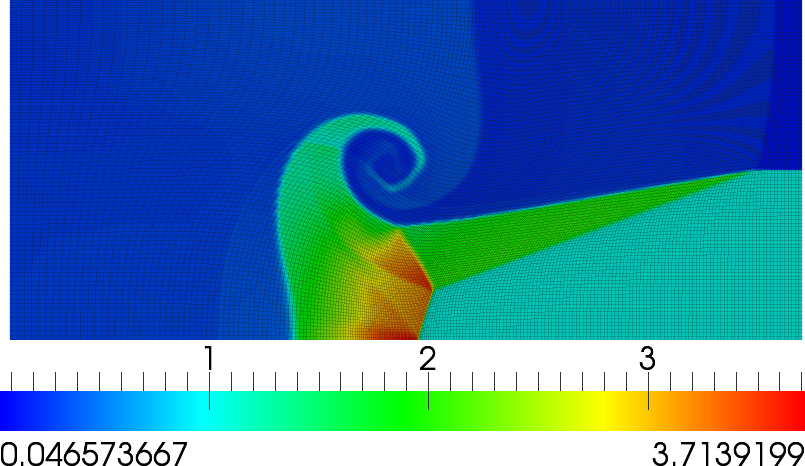
\includegraphics[width=0.8\textwidth]{figs/TriplePt/Q2-4-density-nolimiter.png}\\
\end{center}
\end{column}
\end{columns}
}
\end{frame}
\begin{comment}
This is the triple point shockwave with Q2Q1 elements. We ran this in ALE mode, with
remap every 20 timesteps to demonstrate that this technique is not exclusive to a
Lagrangian framework. In fact, the initial paper by Persson and Peraire was for
Eulerian simulations.

You can see that our smoothness indicator does a decent job at picking out the main
features of the flow and isolating the viscosity to those regions.
\end{comment}


%===============================================================================
% NEW SLIDE
%===============================================================================
\begin{frame}\frametitle{Conclusions}
\begin{exampleblock}{What have we done?}
\begin{itemize}
\item Current implementation of artificial viscosity limits our convergence to first order.
\item Need a limiter which turns off viscosity for smooth flow.
\item Project velocity onto a lower order space and measure the difference as a shock detector.
\item Turn off viscosity any time the detector falls below a certain threshold.
\end{itemize}
\end{exampleblock}
\begin{exampleblock}{Does it make a difference?}
\begin{itemize}
\item We recover high order convergence for Taylor-Green after we achieve sufficient resolution.
\item For most shock problems we eliminate excess viscosity.
\item Our limiter eliminates too much viscosity in the Noh problem.
\item Field variables appear little changed in other problems.
\end{itemize}
\end{exampleblock}
\begin{exampleblock}{What can we do to improve on these results?}
\begin{itemize}
\item Consider making $s_0$ and $\kappa$ functions of $h$ and/or $p$.
\item Try using physical mass matrices in $L^2$ projection.
\item Experiment with other trigger variables.
\item Explore the possibility expanding velocity in terms of orthonormal Legendre polynomials.
\item Try using the detector as a viscosity itself, rather than a limiter.
\end{itemize}
\end{exampleblock}
\end{frame}


% \bibliographystyle{plain}
% {\scriptsize
% \bibliography{../DPG.bib}
% }

\end{document}
